Per lo studio delle geometrie molecolari utilizzeremo due approcci diversi: prima tratteremo delle molecole semplici, dopodiché vedremo come sia possibie generalizzare alcune informazioni per studiare molecole più complesse.
\subsection{Lo stato di promozione del carbonio}
Consideriamo la molecola del metano \ce{CH_4}. In essa il carbonio è legato a quattro atomi di idrogeno, per cui la sua valenza è pari a 4.

La configurazione elettronica del carbonio nello stato fondamentale però è
$$\text{C} \quad 1s^22s^22p_x^12p_y^12p_z^0 \quad \subshell{1s:2} \; \subshell{2s:2} \; \subshell{2p:110}$$
Nota: l'avere scritto  un elettrone nel 2p$_x$, uno nel 2p$_y$ e zero nel 2p$_z$ è stata una nostra scelta: potevamo scegliere che fosse vuoto il 2p$_x$ e occupati 2p$_y$ e 2p$_z$, oppure che fosse vuoto il 2p$_y$ e occupati 2p$_x$ e 2p$_z$

Avendo solo due orbitali parzialmente occupati, questa configurazione ci porta a pensare che il carbonio abbia valenza 2, in contrasto in quasi tutti i suoi composti il carbonio è tetravalente.

Per spiegare la valenza 4, si è pensato che uno degli elettroni degli orbitali 2s (che col 2p sono i livelli di valenza) possa essere promosso al restante orbitale p vuoto in modo tale che la confogurazione elettronica del carbonio in questo nuovo stato, detto di promozione, sia

$$\text{C} \quad 1s^22s^12p_x^12p_y^12p_z^1 \quad \subshell{1s:2} \; \subshell{2s:1} \; \subshell{2p:111}$$

Lo stato di promozione tuttavia riesce a giustificare solo la valenza 4 del carbonio, ma non la geometria del metano: sperimentalmente per esso si misurano quattro legami tutti uguali, ma se abbiamo pensato di avere parzialmente occupati un orbitale s e tre orbitali p non ce li aspetteremmo tali, in quanto gli orbitali p sono direzionali (in particolar modo sono diretti lungo gli assi cartesiani), mentre l'orbitale s è a simmetria sferica. Inoltre i legami dovuti ai tre orbitali p dovrebbero stare a 90° l'uno dall'altro, ma nei fatti gli angoli sono di 109.5°.
\subsection{La teoria dell'ibridizzazione sp}
A questo punto interviene la teoria dell'ibridizzazione, ossia si parla di \textbf{orbitali ibridi} sp: si pensa che i tre orbitali p e l'orbitale s si mescolino fra loro per dare luogo a quattro orbitali identici, a meno della diversa orientazione, i quali si chiamanno ibridi proprio perché hanno sia carattere s che carattere p.

Gli orbitali sp possiedono un lobo molto più grande dell'altro, ciò è dovuto al fatto che le funzioni d'onda degli orbitali p hanno un segno che segue quello dell'asse lungo cui sono orientati, e in particolare hanno un lobo sul semiasse positivo e uno sul semiasse negativo. Quando li combiniano al 2s che è assunto positivo, avremo una somma per il lobo positivo e una differenza per il quello negativo, da cui segue un rafforzamento della funzione lungo la parte positiva e un decremento lungo quella negativa. Spesso addirittura il lobo piccolo viene trascurato. Inoltre, per comprendere meglio l'orientazione di questi orbitali, il lobo lungo la parte positiva dell'asse viene stilizzato come una goccia allungata:

\begin{figure}[htp]
    \centering
    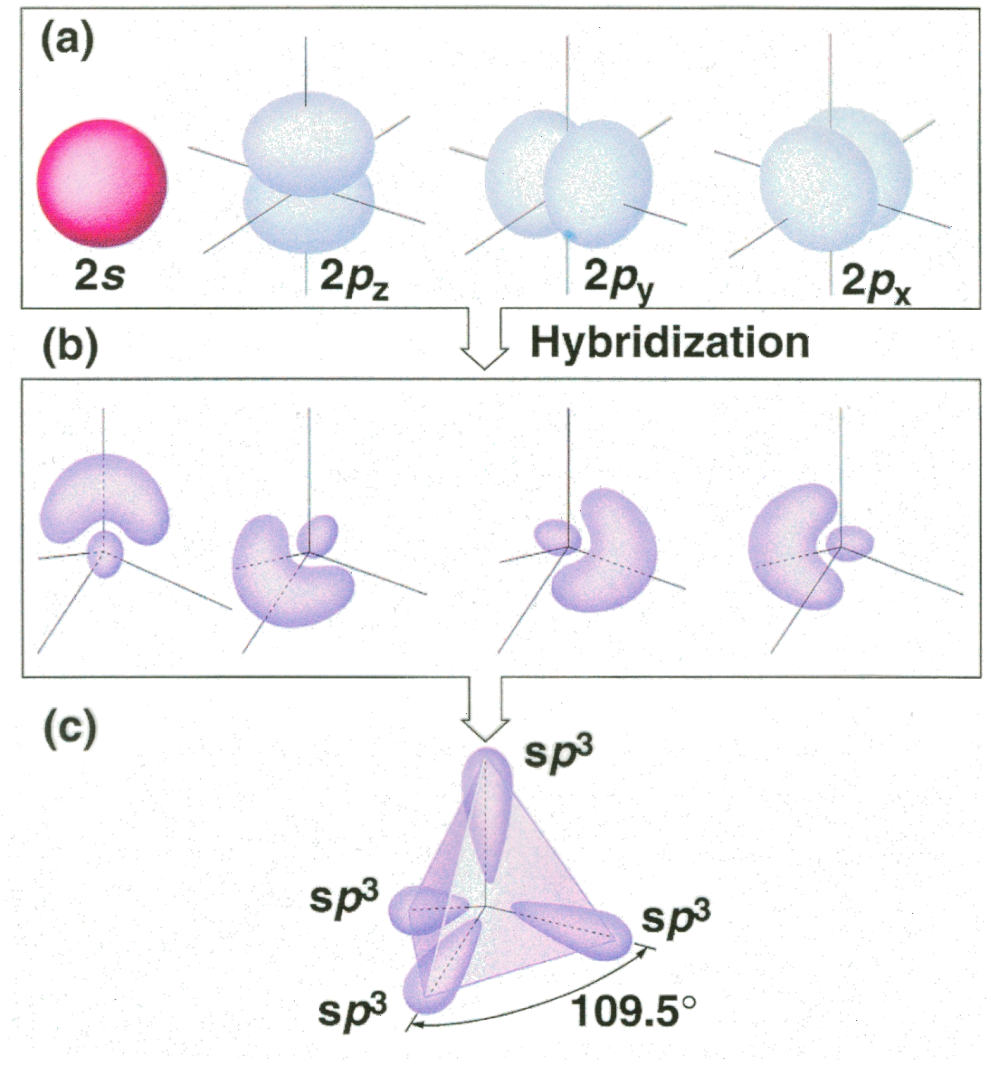
\includegraphics[scale=.5]{immagini/orbitali-sp3.png}
\end{figure}
\newpage
Stilizzandoli diventa evidente che gli orbitali ibridi del carbonio sono orientati lungo i vertici di un tetraedro in cui al centro viene posto il carbonio con i suoi 4 orbitali, i quali formano angoli di 109.5° tra loro.

Avendo mescolato 4 orbitali atomici, ci aspettiamo 4 orbitali ibridi, che nei fatti osserviamo. Essi si chiamano ibridi sp$^3$, dove il 3 indica il numero di orbitali p e non il loro riempimento. 

Con questa teoria dell'ibridazione riusciamo a giustificare la geometria del metano, in quanto ognuno di questi orbitali interagirà con un atomo di idrogeno, creando quattro legame identici
\subsection{Ibridizzazione sp$^2$}
Immaginiamo ora che solo 2 orbitali p si mescolino con l'orbitale s, mentre il terzo resti rigorosamente atomico. In questo modo vengono fuori tre orbitali ibridi detti sp$^2$.

Le molecole in cui il carbonio mostra questo tipo di ibridazione sono planari, cioè gli orbitali giacciono tutti sullo stesso piano e se stilizziamo gli orbitali ci accorgiamo che questi puntano a 120° l'uno dall'altro. Si dice che hanno geometria "trigonale planare". Inoltre, perpendicolarmente a questo piano, abbiamo un orbitale p non coinvolto nell'ibridizzazione, il quale però mantiene un elettrone (vale ancora il discorso dello stato di promozione, altrimenti non potremmo spiegare la tetravalenza)
\subsection{Ibridizzazione sp}
Immaginiamo di mescolare sono uno dei tre orbitali 2p con l'orbitale 2s: otterremo due orbitali ibridi sp. Essi, se stilizzati, mostrano che i lobi giacciono su una linea, quindi tra loro gli angoli sono di 180°. Quindi la geometria è lineare.

I due orbitali p non ibridizzati saranno perendicolari all'asse, e conterranno un elettrone ciascuno.
$$
\schemestart
\chemfig{*6(=-=-=-=)}
\arrow{<->}
\chemfig{*6(-=-=-=)}
\quad
\text{oppure}
\quad
\chemfig{**6(------)}\
\schemestop
$$